\documentclass[tekniskrapport/tech.tex]{subfiles}

\begin{document}

\section{Fjärrklient}
Fjärrklienten fungerar som ett användargränssnitt och har även en
viktig roll i utförandet av uppdrag.

\subsection{Funktion}
Fjärrklientens uppgift är att bidra med ett gränssnitt till användaren för att
kontrollera och se bilens position, samt skapa och skicka instruktioner till
bilen utifrån användarens uppdrag.

\subsection{Gränssnitt} Gränssnittet ska tillåta användaren att välja antingen
autonom eller manuell körning. Vid manuell körning skickas styrkommandon till
taxin när användaren trycker på piltangenterna. Vid autonom körning ska
gränssnittet tillåta användaren att mata in en karta samt ange startnod och
destinationsnod. 

\subsubsection{Kartpanel}
I kartområdet i gränssnittet kan användaren skapa noder och bågar som ska
representera kartan som bilen ska köra. Det sker genom att flytta musen dit man
vill sätta en nod och sedan välja nodtyp. Gränssnittet räknar ut musens
position på kartan och skapar sedan ett nodobjekt på den postitionen.  Ett
bågobjekt skapas genom att klicka startnod och slutnod för bågen.  Bågen får då
dessa start- och slutnoder associerat till sig.  Gränssnittet skall även visa
taxins position under aktiva uppdrag. Det uppnås genom att kolla på vilket
nästa uppdrag är och vilka noder som finns i den kortaste vägen till punkten,
därefter ignorerar den alla tomma noder och markerar de befintliga kanterna
mellan noderna som uppdraget tar hänsyn till  med en rosa färg. När kommandot
är slutfört så minskar listan av kommandon och nästa segment på kartan kan
markeras.

\subsubsection{Kommandorad}
Längst ned i gränssnittet finns en kommandorad där det går skicka kommandon
direkt till kommunikationsmodulen utan att använda någon grafisk funktion.
Kommandot är formaterat precis som det skrivs in i fältet.

\subsubsection{Sensorpanel}
Här hämtas och presenteras alla sensorvärden som grännsittet får genom att be
kommunikationsmodulen om dessa värden. Svaret formateras därefter för att vara
lättläsligt och lämpliga etiktetter läggs till. Gränssnittet visar nuvarande
mätvärden från bilen genom att fråga kommunikationsmodulen efter värdena FRONT,
RIGHT, SPEED, DISTANCE och ERROR. Dessa motsvarar avstånd till närmaste objekt
framåt avstånd till objekt åt höger, hastighet angivet i m/s och felvärde
respektive. 

\subsubsection{Manuell styrning}
När manuellt körläge är aktiverat kopplas piltangenterna till kommandon för att
köra fram, bak, höger och vänster. När en knapp sedan trycks ned skickas
motsvarande kommandot till kommunikationsmodulen som sedan får bilen att röra
på sig.

\subsubsection{Autonom styrning}
Vid autonom körning följer bilen den listan av kommandon som fjärrklienten
skickar i form av uppdraget.

\subsubsection{Ansluta till kommunikationsmodulen}
Genom att mata in ip-addressen till kommunikationsmodulen i gränssnittet erhålls
en anslutning utifrån protokollet TCP. När en anslutning är upprättad går det
att använda alla funktioner som beror på en konstant anslutning till
kommunikationsmodulen.

\subsubsection{Spara och öppna kartor}
Genom gränssnittet går det att både spara och öppna kartor som skapats. Det
sker genom att gränssnittet sparar en kodrepresentation av alla objekt i
kartan. Filen kan sedan läsas in och återskapas i gränssnittet.

\subsubsection{Modifiering av reglerparametrar}
Med användargränsnittet går det att modifiera reglerparametrarna. Värden matas
in fönstret som dyker upp när man väljer mostvarande menyval. Värdena skickas
med hjälp av motsvarande kommando för att ändra konstanterna K-proportionell
och K-derivata för både rotation och hastighet.

\subsubsection{Skapa kommandon för uppdrag}
Fjärrklienten ska utifrån den inmatade kartan och destinationen räkna ut den
kortaste vägen med hjälp av Djiktras algoritmen och utifrån vägen skapa en
lista av kommandon som sedan skickas till bilen. Bilen kan då genom att utifrån
kommandona nå destinationen.

\subsection{Mjukvaruimplementation}
Fjärrklienten kommer implementeras i Python och bestå av två olika trådar. En
för det grafiska gränssnittet samt en huvudtråd för allt annat. Ett
flödesdiagram för fjärrklienten kan ses i bilaga \ref{flow:remote}.

\subsubsection{Filstruktur}
Fjärrklienten byggs upp av följande filer

\begin{labeling}{wwww}
	\item[gui.py] - Motsvarar det grafiska gränssnittet
	
	\item[remote.py] - Beskriver hur klienten kommunicerar med
		kommunkationsmodul via en socket.

	\item[worker.py] - En arbetare som sköter synkronisering av
		fjärrklientens två trådar
	
	\item[tasks.py] - Här definieras kommandon som fjärrklienten kan skicka
		till servern. Den definerar en stack av köer och en kö av
		färdigställda kommandon.  Detta används främst av workern och
		det grafiska gränssnittet.
    
    \item[course.py] - Hanterar översättningen av noder till uppdrag. Utifrån
    en lista av noder skapas en lista av strängar som beskrivet i sektion
    \ref{sec:mission}

    \item[main.py] - Här är fjärrklientens huvudloop som initierar de två
    trådarna för klient och gui.

\end{labeling}
Relationen mellan dessa mjukvarumoduler beskrivs i figur \ref{boxclient}

\begin{figure}[h]
\centering
	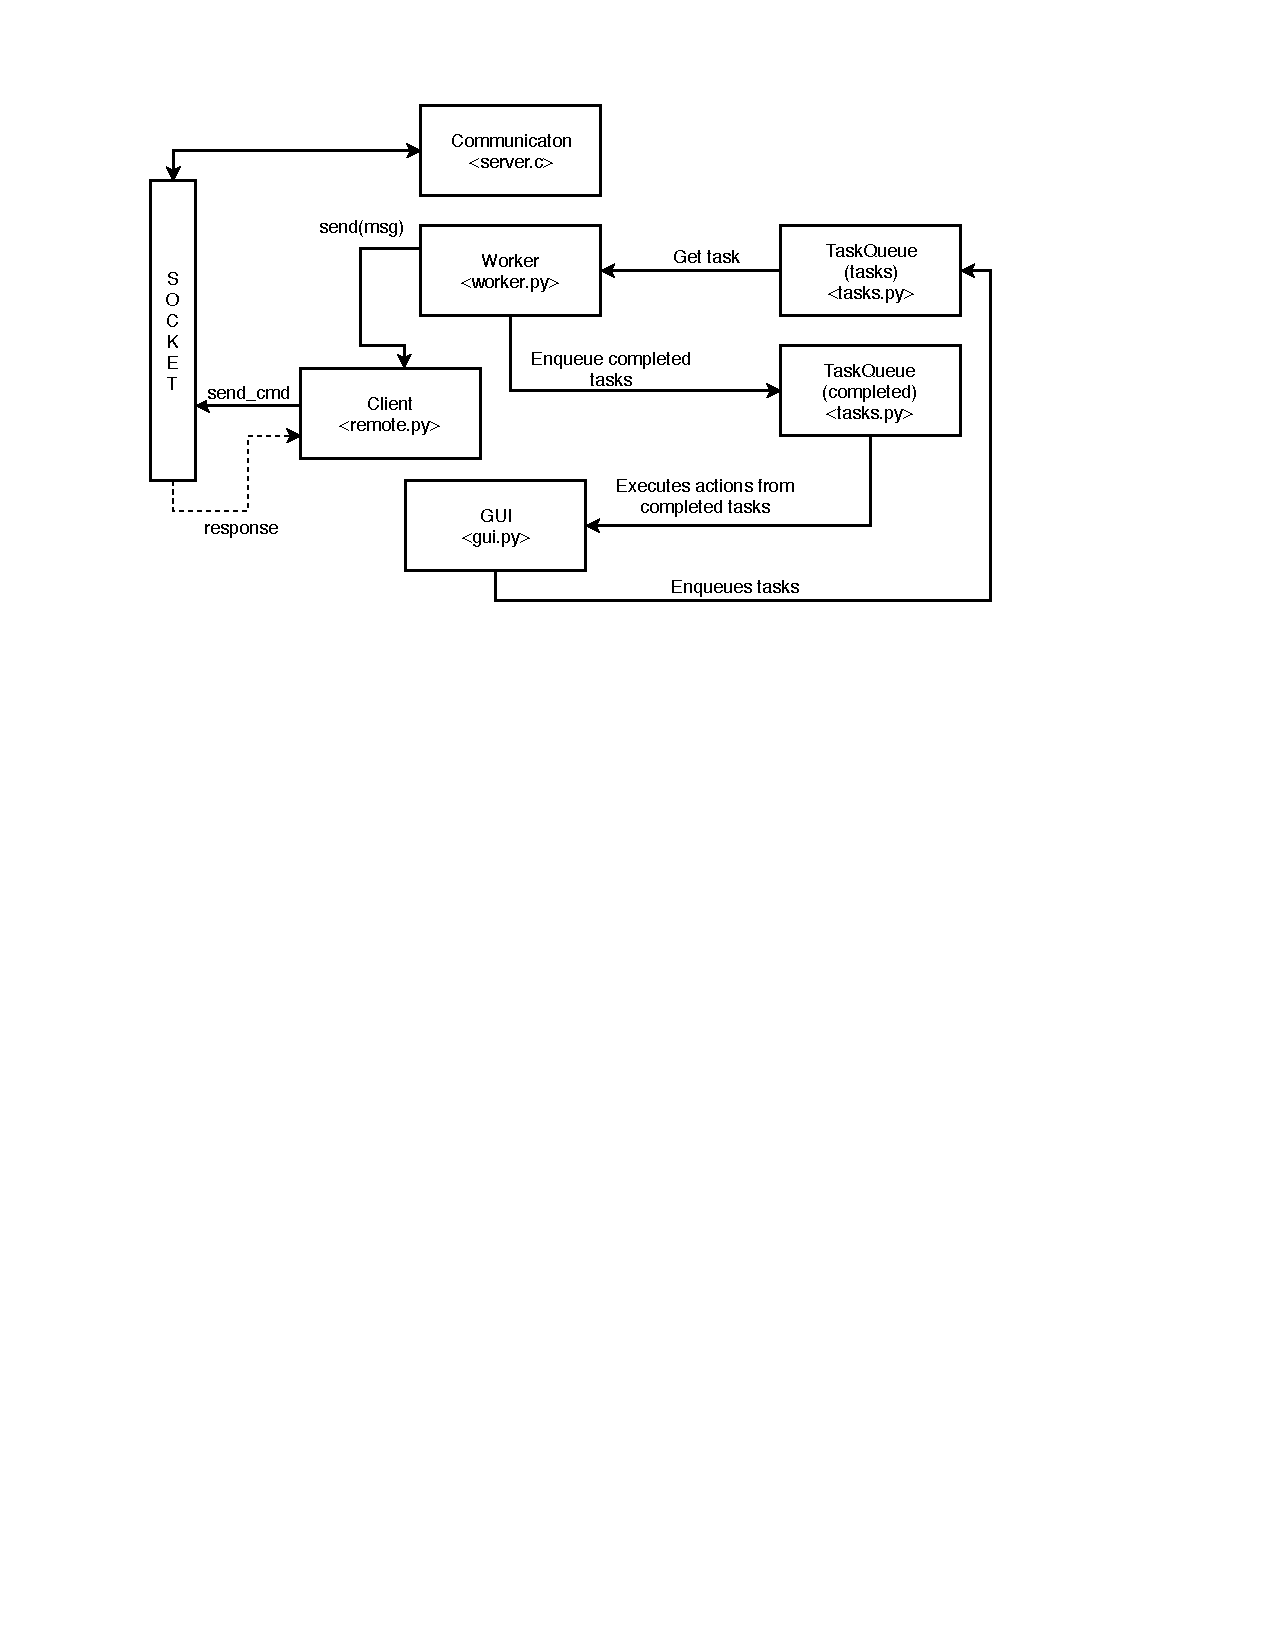
\includegraphics[width=0.6\linewidth]{\figures/client-box-line-diagram.pdf}
	\caption{Ett låd-diagram som beskriver relationen mellan GUI,
	workern och klienten som pratar med servern}
	\label{boxclient}
\end{figure} 

\subsubsection{Trådar}
Programmet skall köras parallellt med två trådar för att förhindra att
gränssnittet fryser för användaren. Programmet kommer behöva vänta på svar från
taxin samt utföra längre beräkningar vilket innebär att programmet kanske inte
hinner uppdatera gränssnittet tillräckligt ofta om det endast använder en tråd.
Synkroniseringen av dessa två trådar sköts av en worker som innehåller en stack
av tupler som består av en task och dess argument och en kö av tupler med
färdiga tasks och responssträng från servern. Stacken och kön är en delad resurs
mellan workern och GUI. GUI och workern körs vardera som en separat tråd. En
task motsvarar ett kommando och dess argument som klienten ska skicka till
kommunikationsmodulen. Det grafiska gränssnittet köar en task i stacken när
användaren utnyttjar en funktion i gränssnittet som kräver kommunikation med
servern. Ett exempel är när användaren har satt ett uppdrag och exekverar
uppdraget. När ett uppdrag sätts så behöver klienten skicka en sekvens av
kommandon till servern, klienten får indirekt en sekvens av kommandon från det
grafiska gränssnittet. Detta sker genom att det grafiska gränssnittet köar i
stacken en tuple bestående av \emph{tasken} SEND\_MISSION och dess argument.
Därefter kommer workern till slut att plocka ut tasken ur stacken och se till
att klienten skickar den korresponderande kommandot till sockeln. Om
överföringen lyckades så kommer klienten att få ett svar. Detta svar skickas
tillbaka till workern som därefter markerar tasken som färdig och köar tasken
och svaret som en tuple i kön med färdiga tasks. Som i figur \ref{boxclient} så
kan det grafiska gränssnittet hämta svaret från tasken genom att avköa den
färdiga tasken och läsa av svaret. Det är på detta sättet det grafiska
gränssnittet kan hämta värden som styrparametrar och distans körd. Denna
procedur förklaras bättre i figur \ref{sequenceremote}.



\begin{figure}[h]
\centering
	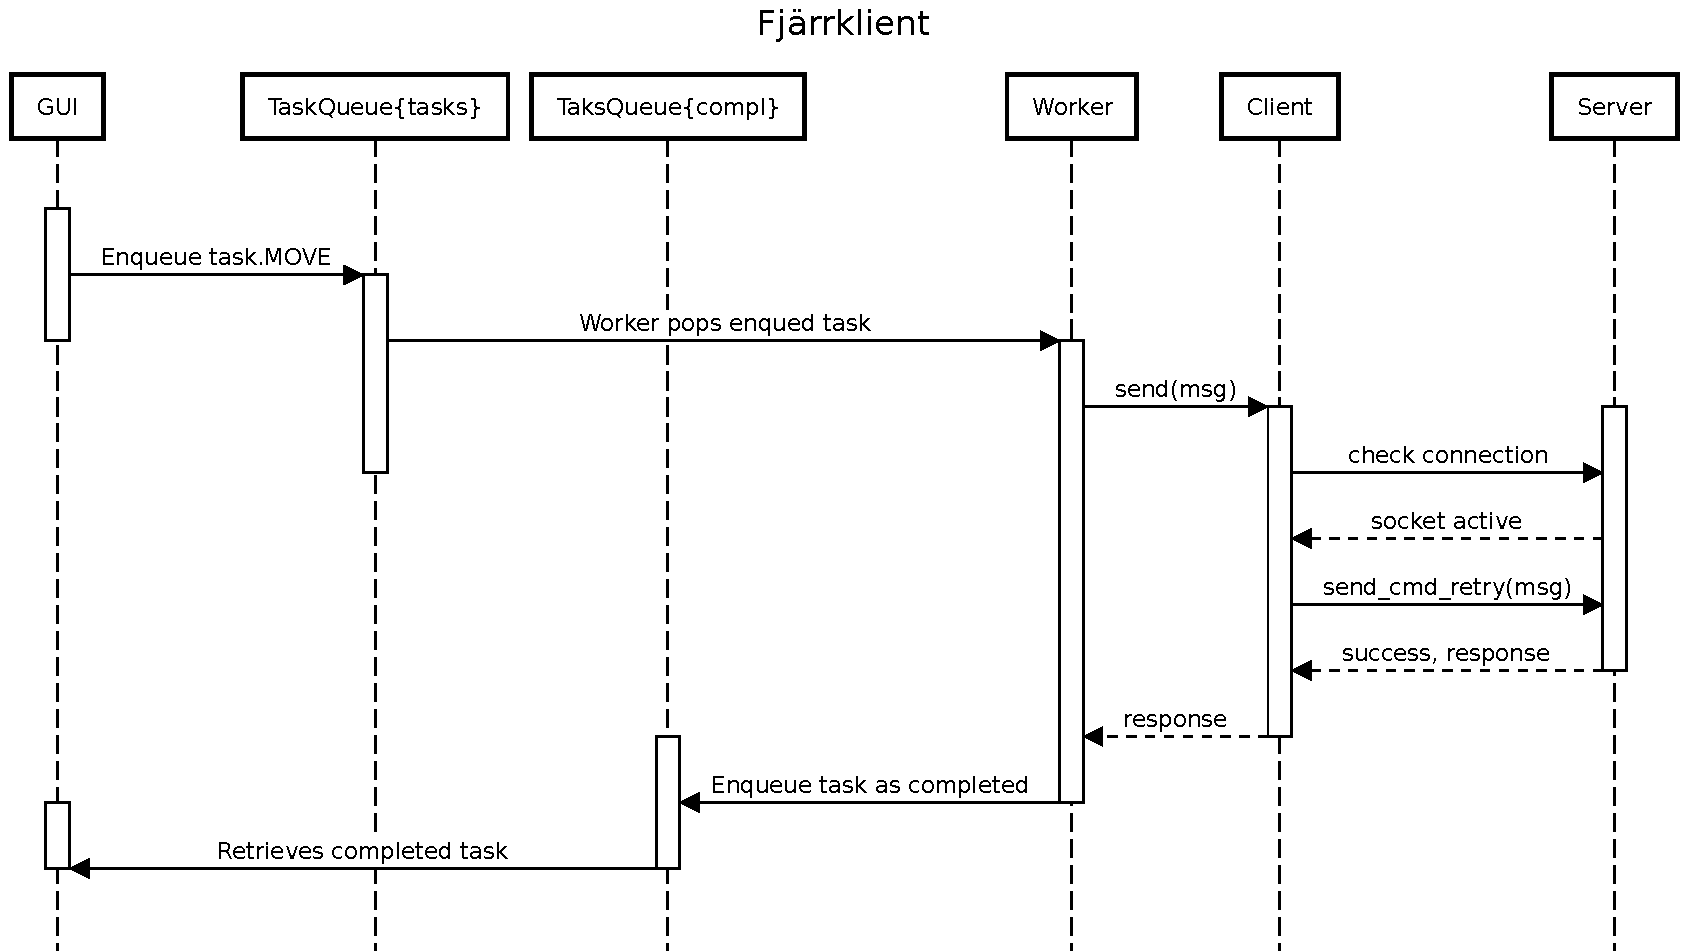
\includegraphics[width=0.6\linewidth]{\figures/SequenceDiagramClient.pdf}
	\caption{Ett sekvensdiagram som beskriver vad som händer när användare trycker
    piltangent upp under fjärrstyrning}
	\label{sequenceremote}
\end{figure}

I figur \ref{sequenceremote} fjärrstyr användaren bilen genom att trycka
piltangent upp. Det är antaget att fjärrklienten och bilen har en anslutning
till sockeln och att överföring mellan klient och bil inte misslyckades. Det
grafiska gränssnittet köar tasken TASK_MOVE i stacken när användaren trycker
piltangent uppåt. Workern hämtar sedan tasken från stacken. Workern bearbetar
tasken och formaterar om dom till en sträng som motsvarar ett kommando. Workern
säger sedan till klienten att skicka kommandot till kommunikationsmodulen och
samtidigt väntar workern på att klienten tills klienten har fått ett svar från
sockeln. Klienten vidarebefodrar svaret till workern och workern markerar tasken
som färdig genom att köa den till kön med färdiga tasks. Enkelriktningen av uppgiftern
gör denna procedur trådsäker.


\subsubsection{Karta och uppdrag}
\label{sec:mission}
Kartan representeras med en riktad graf där varje nod motsvarar en stopplinje
av tejp i vägfältet. Rondeller representeras av infart- och utfartsnoder som
med bågarna bildar en cykel. En båge representerar en enkelriktad körfil från
en stopplinje eller rondell till en annan stopplinje eller rondell. Den här
grafen representeras i sin tur av nedanstående datastrukturer.

% datastrukturer
\begin{labeling}{wwww}
    \item[Karta] Kartan utgörs av en lista med noder.

    \item[Nod] En nod är en klass som består av en nodtyp och en lista
        av utgående bågar. Det finns fem olika nodtyper; stopplinje,
        parkeringsficka, rondellinfarter, rondellutfarter och tomma noder. 

    \item[Båge] En båge är en klass som består av en startnod, en slutnod och
    en kostnad (längd).
        
\end{labeling}
Ovanstående datastrukurer är valda för att göra det smidigt att räkna ut den
närmaste vägen med Dijkstras alogritm. Med algoritmen utgår man från en nod och
jämför alla dess grannar. Med ovanstående struktur kan man utgå från startnoden
och därefter rekursivt gå igenom nodens alla grannar och grannar av grannar.

När en närmaste väg har bestämts, innan en kö av kommandon skapas måste tomma
noder filtreras ut ur vägen. Sedan kan en kö av kommandon skapas. Detta görs
genom att iterera varje nod i vägen och lägga till ett av kommandona nedan för
varje nodtyp. Hur taxin agerar vid varje kommando är specificerat i sektion
\ref{sec:comm-mission}.

\begin{labeling}{wwwwwwwwww}
\item[Stopplinjer] {\commStop} om markerad som destination/deldestination,
annars \commIgnore.

\item[Parkeringsfickor] {\commPark} om markerad som destination/deldestination,
annars \commIgnore 

\item[Rondellinfarter] En \commEnter

\item[Rondellutfarter] En {\commContinue} för varje
avfart den ska passera och slutligen en \commExit.

\end{labeling}
För att kunna avgöra vilken avfart taxin ska ta i en rondell är det viktigt att
de utgående bågarna i rondellens nod är sorterade i samma ordning som
avfarterna är placerade i den riktiga banan.

\end{document}
